\chapter{Estudio, Simulación y Validación de los IP Cores Generados} \label{sec:simsec}

En este capítulo se describen los ensayos de verificación y validación de los IP
Cores generados durante el desarrollo del presente trabajo de tesis. 

\section{Estrategia de simulación, verificación y validación}

Durante el desarrollo de este trabajo se verificó el funcionamiento de cada módulo a través de
simulaciones en verilog comprobando su correcto funcionamiento.

Dada la imposibilidad de ensayar todos los casos, por temas de tiempo, se diseñaron casos de prueba
específicos que son una muestra representativa del conjunto total.

Una vez integrada cada arquitectura se realizaron ensayos de verificación y validación. Mediante
bancos de prueba en verilog se procesaron señales características y se compararon con el resultado de
realizar el mismo procesamiento utilizando Matlab para comprobar el correcto funcionamiento de las
arquitecturas finalizadas. 

Para caracterizar las diferentes arquitecturas se eligieron las siguientes métricas:

\begin{itemize}
  \item Error máximo $\equiv$ $\Vert error \Vert_\infty$
  \item MSE $\equiv$ $\Vert error \Vert_2$
  \item Distorsión Total Armónica
\end{itemize} 

Una vez verificado el funcionamiento a nivel general corroborando que transforma señales conocidas
en sus transformadas y antitransformadas correspondientes, se realizaron ensayos de caracterización
mediante simulaciones a través de bancos de prueba en verilog donde se analizó iterativamente el
funcionamiento de las arquitecturas para obtener parámetros de caracterización como la distorsión
total armónica y una métrica del error de la arquitectura tomando como referencia el procesamiento
de las mismas señales en Matlab.

Se realizaron simulaciones para diferentes tamaños de palabra y cantidad de puntos. Para la cantidad
de bits por palabra se utilizaron los valores de 12 y 16 bits. Estos valores fueron seleccionados
teniendo en cuenta por un lado que 16 bits es un valor standard de codificación y permite la comparación
directa con unidades de cómputo en otros lenguajes como C++, y 12 bits por ser un valor común en lo
que se refiere a transmisiones OFDM. En cuanto a la cantidad de puntos a procesar se realizaron
simmulaciones para $1024$ y $4096$ puntos, al ser cantidades de puntos que pueden procesarse tanto
con la arquitectura radix-2 como con la radix-4.

Todas las simulaciones fueron realizadas utilizando \textit{Modelsim} y \textit{gtkwave}, ambos
mencionados en la sección \ref{sec:herrSec}, para la visualización de las señales resultantes.

\section{Simulación y verificación de los módulos individuales}

Al finalizar la implementación de cada módulo se realizaron pruebas elementales de funcionamiento
utilizando bancos de prueba escritos en verilog donde se buscó verificar que cada módulo cumpla con su
función.

En este sentido los módulos sobre los que se realizaron mayores pruebas son los módulos
multiplicadores, tanto el módulo cordic como el multiplicador complejo.
También se realizaron ensayos de funcionamiento durante el desarrollo de las unidades de control
para depurar la sincornización correcta de las señales de control.

Una vez finalizados los
ensayos y simulaciones con resultados satisfactorios se procedió a la integración de las
arquitecturas.

\section{Simulación y validación de las arquitecturas completas}

Los IP cores generados como resultado del desarrollo del trabajo de tesis fueron sometidos a
simulaciones y ensayos para verificar su correcto funcionamiento de acuerdo a los requerimientos
planteados y obtener cotas de error y distorsión para validar el desarrollo.

\subsection{Procesamiento de señales patrón} \label{sec:enspatron}

Se realizaron una serie de simulaciones utilizando señales patrón cuyas transformadas de Fourier son
conocidas de forma de validar el funcionamiento de las arquitecturas. Para cada señal utilizada se
presenta un gráfico con el resultado de la simulación superpuesto al resultado de realizar la
transformada de Fourier sobre la misma señal utilizando Matlab.
Las arquitecturas se ensayan utilizando un ancho de palabra de $16$ bits, para $4096$ puntos.

\subsubsection{Delta en componente `0'}

Utilizando como entrada una señal compuesta por un único pulso en la primer posición debe dar como
resultado una señal continua de valor constante.

La entrada consistió en
una señal discreta de $4096$ puntos representando el muestreo de una delta en la componente $0$.

En la figura \ref{fig:outDelta0} se observan las salidas obtenidas utilizando ambas arquitecturas
tanto con el multiplicador complejo como con el rotador cordic. En cada gráfico se superpone la
salida de la arquitectura, representada por la señal \textit{core} en los gráficos, a la salida de
realizar la misma fft utilizando precisión de punto flotante como referencia.

\begin{figure}[htbp!]
        %\centering
        \advance\leftskip-1.5cm
        \begin{subfigure}{0.6\textwidth}
        \includegraphics[width=9cm]{./figures/r2_delta0_16_4096_mul.png}
        \caption{Radix 2, multiplicador complejo}
        \end{subfigure}%
        \begin{subfigure}{0.6\textwidth}%\centering
        \includegraphics[width=9cm]{./figures/r2_delta0_16_4096_cor.png}
        \caption{Radix 2, rotador cordic}
        \end{subfigure} 
        \begin{subfigure}{0.6\textwidth}%\centering
        \includegraphics[width=9cm]{./figures/r4_delta0_16_4096_mul.png}
        \caption{Radix 4, multiplicador complejo}
        \end{subfigure}%
        \begin{subfigure}{0.6\textwidth}%\centering
        \includegraphics[width=9cm]{./figures/r4_delta0_16_4096_cor.png}
        \caption{Radix 4, rotador cordic}
        \end{subfigure}
        \caption{Respuestas a una delta en la componente $0$ para las arquitecturas radix-2 y
        radix-4}
        \label{fig:outDelta0}
\end{figure}

\subsubsection{Delta}

La transformada de Fourier de una delta debe dar un seno o un coseno cuya frecuencia está
directamente relacionada con la posición del pulso.

La entrada utilizada para este ensayo consistió en
una delta ubicada en la componente $6$ del vector de $4094$ puntos.

En la figura \ref{fig:outDelta7} se muestran las salidas obtenidas de ambas arquitecturas tanto con
el multiplicador complejo como el rotador cordic. En cada gráfico se superpone la
salida de la arquitectura, representada por la señal \textit{core} en los gráficos, a la salida de
realizar la misma fft utilizando precisión de punto flotante como referencia.

\begin{figure}[htbp!]
        %\centering
        \advance\leftskip-1.5cm
        \begin{subfigure}{0.6\textwidth}
        \includegraphics[width=9cm]{./figures/r2_delta7_16_4096_mul.png}
        \caption{Radix 2, multiplicador complejo}
        \end{subfigure}%
        \begin{subfigure}{0.6\textwidth}%\centering
        \includegraphics[width=9cm]{./figures/r2_delta7_16_4096_cor.png}
        \caption{Radix 2, rotador cordic}
        \end{subfigure} 
        \begin{subfigure}{0.6\textwidth}%\centering
        \includegraphics[width=9cm]{./figures/r4_delta7_16_4096_mul.png}
        \caption{Radix 4, multiplicador complejo}
        \end{subfigure}%
        \begin{subfigure}{0.6\textwidth}%\centering
        \includegraphics[width=9cm]{./figures/r4_delta7_16_4096_cor.png}
        \caption{Radix 4, rotador cordic}
        \end{subfigure}
        \caption{Respuestas a una delta en la componente $7$ para las arquitecturas radix-2 y
        radix-4}
        \label{fig:outDelta7}
\end{figure}

\subsection{Medición del error}

Para medir el error de procesamiento de las arquitecturas se utilizó como parámetro el resultado de
realizar el mismo procesamiento mediante Matlab, ya que al utilizar precisión en punto flotante de
64 bits provee un buen contraste para la precisión en entero de 12 o 16 bits de las arquitecturas.

Para obtener un parámetro comparable del error
se obtienen dos métricas basadas en el cálculo de la norma de los vectores de señal y de error.
Definiendo la norma $p$ de un vector $x$ de tamaño $N$ como:

\begin{equation}
\Vert\vec{x}\Vert_p = \sqrt[p]{x[1]^p+x[2]^p+\ldots+x[N]^p}
\label{eq:normap}
\end{equation}

Se toma el error relativo en base a dos normas calculadas según (\ref{eq:normap}), dando las
métricas $E_\infty$ y $E_2$ como sigue:

\begin{equation}
E_\infty = MAX\left(\frac{ X_o[n] - X_{dut}[n]}{X_o[n]}\right)
\label{eq:norma1}
\end{equation}

\begin{equation}
E_2 = \left\Vert\frac{X_o[n] - X_{dut}[n]}{X_o[n]}\right\Vert_2
\label{eq:norma2}
\end{equation}

permitiendo estas métricas tener una medida del error ponderable y comparable.

Teniendo en cuenta que las arquitecturas implementadas se comportan como sistemas no lineales, para
obtener métricas confiables de error cada simulación consistió en $1024$ corridas con vectores de
entrada generados aleatoriamente en cada corrida. Se calcularon las métricas $E_\infty$ y $E_2$ para
cada corrida y luego se promedió el valor de las métricas de todas las corridas obteniendo así los
valores de error de cada simulación.

En la figura \ref{fig:errorsim} se presenta un diagrama de flujo del \textit{script} de simulación para la
estimación del error. 

\begin{figure}[htb!]
        \centering
        \includegraphics[width=4cm]{./figures/error_sim.png}
        \caption{Diagrama de flujo de la simulación para la estimación del error}
        \label{fig:errorsim}
\end{figure}

Se simularon $8$ esquemas distintos para cada arquitectura, donde se alternaron los dos módulos
multiplicadores, la unidad cordic y el multiplicador complejo, con dos anchos de palabra, $12$ y
$16$ bits, para dos cantidades de puntos diferentes, $1024$ y $4096$.
Además se realizaron dos simulaciones más utilizando una unidad de cómputo de FFT desarrollada por
terceros ampliamente difundida en lenguaje C++, conocida como KISS FFT \cite{KISSFFT},
con precisión de punto fijo de 16 bits.
%TODO métrica s de error

En la tabla \ref{table:errorInf} se muestran los resultados de las mediciones de error utilizando la
métrica $E_\infty$, mientras que en la tabla \ref{table:error2} se muestran las mediciones de error
utilizando la métrica $E_2$.

\begin{table}[htb!]
\begin{tabular}{l c c c c}
 & \textbf{1024, 12 bits} & \textbf{1024, 16 bits} & \textbf{4096, 12 bits} & \textbf{4096, 16 bits}\\ \hline 
\textbf{Radix-2, cordic} & $0.092$ & $0.006$ & $0.099$ & $0.008 $\\
\textbf{Radix-2, Mult.} & $0.232$ & $0.003$ & $0.340$ & $0.108$\\
\textbf{Radix-4, cordic} & $0.077$ & $0.003$ & $0.074$ & $0.007$\\
\textbf{Radix-4, Mult.} & $0.224$ & $0.002$ & $0.334$ & $0.105$\\
\textbf{Kiss FFT} & $ $ & $0.017$ & $ $ & $0.035$\\\hline
\end{tabular}
\caption{Métrica $E_\infty$ para 1024 realizaciones de cada arquitectura con entradas aleatorias}
\label{table:errorInf}
\end{table}

\begin{table}[htb!]
\begin{tabular}{l c c c c }
 & \textbf{1024, 12 bits} & \textbf{1024, 16 bits} & \textbf{4096, 12 bits} & \textbf{4096, 16 bits}\\ \hline 
\textbf{Radix-2, cordic} & $0.095$ & $0.007$ & $0.116$ & $0.053$\\
\textbf{Radix-2, Mult.} & $0.257$ & $0.004$ & $0.356$ & $0.131$\\
\textbf{Radix-4, cordic} & $0.084$ & $0.002$ & $0.094$ & $0.027$\\
\textbf{Radix-4, Mult.} & $0.258$ & $0.003$ & $0.358$ & $0.126$\\ 
\textbf{Kiss FFT} & $ $ & $0.017$ & $ $ & $0.035$\\\hline
\end{tabular}
\caption{Métrica $E_2$ para 1024 corridas de cada arquitectura con entradas aleatorias}
\label{table:error2}
\end{table}

Se puede ver que el desempeño de las distintas variantes de las arquitecturas es aceptable, incluso
comparado con el algoritmo FFT implementado en C++.

Se puede ver que para $12$ bits el algoritmo cordic produce menor error que el multiplicador
complejo. Esto se debe a que el efecto de la cuantización se hace más evidente en el multiplicador
ya que al implementar los factores de multiplicación correspondientes a cada ángulo, el error de
cuantización es mayor que al utilizar solo el ángulo como en el caso del cordic. Además, el hecho de
realizar una multiplicación entre dos valores con precisión de punto fijo el error del resultado es
mayor que en el caso de sumas y dezplazamientos de una sola palabra como sucede en el cordic.
En cambio, para un tamaño de palabra de $16$ bits la magnitud del error de ambos sistemas de
multiplicación por los twiddle factors es equivalente ya que es menos significativo el error de
cuantización de los factores del multiplicador.

Para reducir el error del multiplicador complejo se debe
aumentar el tamaño de palabra con el que se almacenan los factores correspondientes a cada ángulo,
lo que aumenta el tamaño de memoria utilizada y el tamaño de los registros con los que se realizan
las operaciones. Para reducir el error del rotador cordic se puede aumentar la cantidad de
iteraciones del algoritmo, pero esto tiene como concecuencia un aunmento en el tiempo consumido para
realizar la rotación y un aumento en la memoria destinada a almacenar los valores de
$\arctan(2^{-i})$.

Tambien se puede observar que el error para las arquitecturas de $4096$ puntos es mayor que el error
para las arquitecturas de $1024$ puntos. Esto se debe a que para procesar mayor cantidad de puntos
se requiere mayor cantidad de etapas, lo que lleva a mayor cantidad de operaciones aritméticas que
contienen error, que se acumula y se arrastra de una etapa a la siguiente. De este modo, mientras
más etapas tenga la arquitectura mayor será el error de la misma. Por este mismo motivo las
arquitecturas radix-4 presentan menor error que las radix-2, ya que para la misma cantidad de
puntos poseen menor número de etapas, lo que resulta en menos multiplicaciones. Esto último
representa la principal ventaja de la arquitectura radix-4 por sobre la radix-2 indepenientemente
del tipo de implementación que se utilice.

La diferencia en el error para los dos tamaños de palabras ensayados se debe al error de
cuantización producto de la diferencia de precisión entre los dos tamaños. Mientras que con
$12$ bits la cuantización se da en pasos de $\frac{1}{2^{12-1}} = 4.88 * 10^{-4}$, para $16$ bits es
de $\frac{1}{2^{16-1}} = 3.05 * 10^{-5}$.

También se observa que para $1024$ puntos el error de las arquitecturas iterativas es menor que el
de la Kiss FFT, mientras que para $4096$ puntos el error de las arquitecturas utilizando cordic es
del orden del error de la implementación en C++. Estos resultados verifican que las arquitecturas
resultantes del presente trabajo de tesis son aptas para su uso práctico, al menos en cuanto al
error que producen.\\ 
En cuanto a los resultados de error para las arquitecturas con multiplicador
complejo de $4096$ puntos, se debería aumentar el ancho de palabra de los factores de multiplicación
almacenados en memoria para mejorar las métricas obtenidas.


\subsection{Medición de la distorsión total armónica}

La distorsión total armónica (THD por sus siglas en inglés, Total Harmonic Distortion) es
la aparición de componentes espúreas en la salida de un sistema no lineal al aplicar a la entrada un
tono puro.
En el caso del presente trabajo de tesis el procesamiento de
datos comprende el cómputo de una FFT o iFFT, por lo que la aparición de componentes espúreas tanto en frecuencia como en muestras
temporales debe mantenerse en el nivel míinimo posible ya que puede distorisonar completamente el
resultado del procesamiento, además de ser una medida de la no linealidad del sistema.

La distorsión total armónica se calcula como:

\begin{equation}
THD = \frac{\sum Potencia de los armonicos}{Potencia del tono fundamental} =
\frac{P_1+P_2+\ldots +P_N}{P_0}
\label{eq:THD1}
\end{equation}

Donde $P_0$ es la potencia del tono fundamental de frecuencia $f_0$ y $P_1\ldots P_N$ la potencia de
los armónicos de frecuencia $2*f_0\ldots N*f_0$.

Para obtener una caracterización de la \textit{THD} se utilizó un banco de prueba en verilog que permite
leer como entrada valores complejos listados en un archivo de texto, realizar el cómputo de la FFT
mediante la arquitectura a ensayar y escribir la salida en un archivo de texto. 
La simulación completa se llevó a cabo mediante un \textit{script} en Matlab que crea un archivo de texto que
funciona como entrada de la arquitectura, llama a la simulación de la arquitectura mediante el
banco de prueba descripto y luego procesa la salida de la simulación para hallar el valor de la
\textit{THD}, realizando su transformada de Fourier en un sistema de mayor precisión y analizando
sus componentes.
Para lograr una caracterización lo más completa posible se realizaron simulaciones sucesivas recorriendo de a uno por vez todos los tonos de entrada posibles y registrando el valor de
\textit{THD} para cada uno, de forma de obtener el valor para cada tono de entrada.\\
La forma de calcular la \textit{THD} es la siguiente:

\begin{equation}
THD = 10*\log(\frac{\sum_1^N A_i^2}{A_0^2})
\label{eq:THD2}
\end{equation}

donde $A_i$ es la amplitud de la componente de frecuencia $f_i$, dando el resultado del cálculo en
dB.

En la figura \ref{fig:thdsim} se muestra un diagrama de flujo de la simulación para la estimación de
la \textit{THD}. \textit{Core sim} indica la simulación del IP Core mediante Modelsim, el resto de
las acciones son llevadas a cabo en Matlab.

\begin{figure}[htb!]
        \centering
        \includegraphics[width=4cm]{./figures/thd_sim.png}
        \caption{Diagrama de flujo de la simulación para la estimación de la THD}
        \label{fig:thdsim}
\end{figure}

De este modo se llevaron a cabo 16 simulaciones, combinando los dos valores de tamaño de palabra y
los dos valores de cantidad de puntos, para cada una de las dos arquitecturas desarrolladas
utilizando como unidad de multiplicación por los \textit{twiddle factors} el módulo cordic y el
multiplicador complejo. Además se realizó el mismo análisis para una arquitectura KISS FFT utilizando tamaño de
palabra de 16 bits en punto fijo.
% En las tablas \ref{table:THDprom12} y \ref{table:THDprom16} se muestran la distorsión armónica total 
% promedio para cada una de las configuraciones mencionadas para cada arquitectura separadas por
% tamaño de palabra. El promedio mostrado en dichas tablas se obtuvo descartando los tonos que al ser
% procesados dieron un valor de \textit{THD} interpretado por Matlab como $-\infty$, valor debido al
% que el valor de magnitud de los armónicos es cero.
% 
% \begin{table}[htb!]
% \begin{tabular}{l c c c c}
%  & \textbf{Radix-2 cordic} & \textbf{Radix-2 mult} & \textbf{Radix-4 cord} & \textbf{Radix-4 mult}\\ \hline 
% \textbf{1024 puntos} & $-69.68$ & $-85.84$ & $-70.52$ & $-84.1$\\
% \textbf{4096 puntos} & $-76.51$ & $ -92.23$ & $-77.31$ & $-90.08$\\ \hline
% \end{tabular}
% \caption{THD promedio para tamaño de palabra de 12 bits}
% \label{table:THDprom12}
% \end{table}
% 
% %TODO Modificar tabla con resultados de simulación:
%  \begin{table}[htb!]
% \begin{tabular}{l c c c c c}
% & \textbf{R-2 cordic} & \textbf{R-2 mult} & \textbf{R-4 cordic} & \textbf{R-4 mult} &
% \textbf{Kiss-FFT}\\ \hline
% \textbf{1024 puntos} & $ $ & $-108.72$ & $-92.37$ & $ $ & $-59.48$\\
% \textbf{4096 puntos} & $ $ & $-116.98$ & $ $ & $-116.88 $ & $-52.95$\\ \hline
% \end{tabular}
% \caption{THD promedio para tamaño de palabra de 16 bits}
% \label{table:THDprom16}
% \end{table}

En la figura \ref{fig:r2_thd_1024} se muestra la THD para cada tono utilizado como
entrada, para la arquitectura radix-2 iterativa para 1024 puntos, tanto para 12 bits como para 16 bits de
ancho de palabra, utilizando el rotador cordic y el multiplicador complejo.

\begin{figure}[htbp!]
        %\centering
        \advance\leftskip-1.5cm
        \begin{subfigure}{0.6\textwidth}%\centering
        \includegraphics[width=9cm]{./figures/thd_r2_1024_12_mul.png}
        \caption{Radix 2, multiplicador complejo, 12 bits}
        \end{subfigure}%
        \begin{subfigure}{0.6\textwidth}\centering
        \includegraphics[width=9cm]{./figures/thd_r2_1024_12_cor.png}
        \caption{Radix 2, rotador cordic, 12 bits}
        \end{subfigure} 
        \begin{subfigure}{0.6\textwidth}\centering
        \includegraphics[width=9cm]{./figures/thd_r2_1024_16_mul.png}
        \caption{Radix 2, multiplicador complejo, 16 bits}
        \end{subfigure}% 
        \begin{subfigure}{0.6\textwidth}\centering
        \includegraphics[width=9cm]{./figures/thd_r2_1024_16_cor.png}
        \caption{Radix 2, rotador cordic, 16 bits}
        \end{subfigure}%
        \caption{THD en función del tono de entrada, radix-2 de 1024 puntos}
        \label{fig:r2_thd_1024}
\end{figure}

En la figura \ref{fig:r2_thd_4096} se ven los gráficos de la THD para cada tono utilizado como
entrada, para la arquitectura radix-2 iterativa para 4096 puntos, tanto para 12 bits como para 16 bits de
ancho de palabra, utilizando el rotador cordic y el multiplicador complejo.

\begin{figure}[htbp!]
        %\centering
        \advance\leftskip-1.5cm
        \begin{subfigure}{0.6\textwidth}%\centering
        \includegraphics[width=9cm]{./figures/thd_r2_4096_12_mul.png}
        \caption{Radix 2, multiplicador complejo, 12 bits}
        \end{subfigure}%
        \begin{subfigure}{0.6\textwidth}%\centering
        \includegraphics[width=9cm]{./figures/thd_r2_4096_12_cor.png}
        \caption{Radix 2, rotador cordic, 12 bits}
        \end{subfigure} 
        \begin{subfigure}{0.6\textwidth}%\centering
        \includegraphics[width=9cm]{./figures/thd_r2_4096_16_mul.png}
        \caption{Radix 2, multiplicador complejo, 16 bits}
        \end{subfigure}% 
        \begin{subfigure}{0.6\textwidth}%\centering
        \includegraphics[width=9cm]{./figures/thd_r2_4096_16_cor.png}
        \caption{Radix 2, rotador cordic, 16 bits}
        \end{subfigure} 
        \caption{THD en función del tono de entrada, radix-2 de 4096 puntos}
        \label{fig:r2_thd_4096}
\end{figure}

En la figura \ref{fig:r4_thd_1024} se ven los gráficos de la THD para cada tono utilizado como
entrada, para la arquitectura radix-4 iterativa para 1024 puntos, tanto para 12 bits como para 16 bits de
ancho de palabra, utilizando el rotador cordic y el multiplicador complejo.

\begin{figure}[htbp!]
        %\centering
        \advance\leftskip-1.5cm
        \begin{subfigure}{0.6\textwidth}%\centering
        \includegraphics[width=9cm]{./figures/thd_r4_1024_12_mul.png}
        \caption{Radix 4, multiplicador complejo, 12 bits}
        \end{subfigure}%
        \begin{subfigure}{0.6\textwidth}%\centering
        \includegraphics[width=9cm]{./figures/thd_r4_1024_12_cor.png}
        \caption{Radix 4, rotador cordic, 12 bits}
        \end{subfigure} 
        \begin{subfigure}{0.6\textwidth}%\centering
        \includegraphics[width=9cm]{./figures/thd_r4_1024_16_mul.png}
        \caption{Radix 4, multiplicador complejo, 16 bits}
        \end{subfigure}% 
        \begin{subfigure}{0.6\textwidth}%\centering
        \includegraphics[width=9cm]{./figures/thd_r4_1024_16_cor.png}
        \caption{Radix 4, rotador cordic, 16 bits}
        \end{subfigure} 
        \caption{THD en función del tono de entrada, radix-4 de 1024 puntos}
        \label{fig:r4_thd_1024}
\end{figure}

En la figura \ref{fig:r4_thd_4096} se ven los gráficos de la THD para cada tono utilizado como
entrada, para la arquitectura radix-4 iterativa para 4096 puntos, tanto para 12 bits como para 16 bits de
ancho de palabra, utilizando el rotador cordic y el multiplicador complejo.

\begin{figure}[htbp!]
        %\centering
        \advance\leftskip-1.5cm
        \begin{subfigure}{0.6\textwidth}%\centering
        \includegraphics[width=9cm]{./figures/thd_r4_4096_12_mul.png}
        \caption{Radix 4, multiplicador complejo, 12 bits}
        \end{subfigure}%
        \begin{subfigure}{0.6\textwidth}%\centering
        \includegraphics[width=9cm]{./figures/thd_r4_4096_12_cor.png}
        \caption{Radix 4, rotador cordic, 12 bits}
        \end{subfigure} 
        \begin{subfigure}{0.6\textwidth}%\centering
        \includegraphics[width=9cm]{./figures/thd_r4_4096_16_mul.png}
        \caption{Radix 4, multiplicador complejo, 16 bits}
        \end{subfigure}% 
        \begin{subfigure}{0.6\textwidth}%\centering
        \includegraphics[width=9cm]{./figures/thd_r4_4096_16_cor.png}
        \caption{Radix 4, rotador cordic, 16 bits}
        \end{subfigure} 
        \caption{THD en función del tono de entrada, radix-4 de 4096 puntos}
        \label{fig:r4_thd_4096}
\end{figure}

En la figura \ref{fig:kiss_thd_4096} se ven los gráficos de la THD para cada tono utilizado como
entrada, para la arquitectura KISS FFT en C++ para 16 bits de
ancho de palabra, para 1024 y 4096 puntos.

\begin{figure}[htbp!]
        %\centering
        \advance\leftskip-1.5cm
        \begin{subfigure}{0.6\textwidth}%\centering
        \includegraphics[width=9cm]{./figures/thd_kiss_1024_16.png}
        \caption{Kiss FFT, 1024 puntos}
        \end{subfigure}% 
        \begin{subfigure}{0.6\textwidth}%\centering
        \includegraphics[width=9cm]{./figures/thd_kiss_4096_16.png}
        \caption{Kiss FFT, 4096 puntos}
        \end{subfigure}
        \caption{THD en función del tono de entrada, Kiss FFT}
        \label{fig:kiss_thd_4096}
\end{figure}

Se puede ver en todos los casos que la THD disminuye a niveles casi insignificantes para tonos en el
centro del ancho de banda, subiendo luego a valores más significativos en los tonos en los límites
del ancho de banda.

De los gráficos se puede deducir que el comportamiento de las arquitecturas desarrolladas durante el
trabajo de tesis se comporta de igual manera que el algoritmo implementado en C++, ampliamente
difundido su uso en aplicaciones de procesamiento de señales.

\subsubsection{Efecto de la intermodulación}

La intermodulación es la modulación entre tonos, esto es, la distorsión que produce un tono sobre
los tonos contiguos.
Durante las mediciones de THD se colocó a la entrada un tono puro por vez y se midió los tonos
presentes a la salida. Esta medición no permite ver los efectos de intermodulación ya que esta se produce en presencia de más de un tono a la
entrada.

Para verificar la presencia de efectos significativos de intermodulación se realizaron algunas
mediciones donde se utilizó como señal de entrada un tono puro primero, y luego el mismo tono junto con el tono siguiente. Comparando
las salidas de ambos procesamientos se puede ver si el efecto de la intermodulación es relevante o
puede ser desestimado.

En la figura \ref{fig:two_delta} se muestran los resultados de algunas de estas mediciones. En los
gráficos se superpone el resultado de utilizar un solo tono con el resultado de utilizar como
entrada ese mismo tono y el tono inmediato anterior. Se puede ver que no se generan tonos armónicos
de valor considrable, solo se superponen al espectro original los armónicos generados por el segundo
tono, de magnitud comparable a los armónicos del primer tono.

\begin{figure}[htbp!]
        %\centering
        \advance\leftskip-1.5cm
        \begin{subfigure}{0.6\textwidth}%\centering
        \includegraphics[width=9cm]{./figures/thd_r2_4096_16_mul_450_451.png}
        \caption{Radix 2, multiplicador complejo}
        \end{subfigure} 
        \begin{subfigure}{0.6\textwidth}%\centering
        \includegraphics[width=9cm]{./figures/thd_r2_4096_16_cor_450_451.png}
        \caption{Radix 2, rotador cordic}
        \end{subfigure} 
        \begin{subfigure}{0.6\textwidth}%\centering
        \includegraphics[width=9cm]{./figures/thd_r4_4096_16_mul_450_451.png}
        \caption{Radix 4, multiplicador complejo}
        \end{subfigure}
        \begin{subfigure}{0.6\textwidth}%\centering
        \includegraphics[width=9cm]{./figures/thd_r4_4096_16_cor_450_451.png}
        \caption{Radix 4, rotador cordic}
        \end{subfigure}
        \caption{THD de la respuesta a dos tonos concecutivos}
        \label{fig:two_delta}
\end{figure}

\subsection{Efectos de redondear o truncar en una etapa}

Se realizaron mediciones aplicando escalamientos, redondeo o truncamiento, aplicando primero una
señal aleatoria y se comparó la salida con la respuesta a la misma entrada de la arqutiectura sin
escalar. En la figura \ref{fig:trunnotrunc} se muetra una ampliación de una zona de la salida de
ambas arquitecturas, con y sin escalamiento, a la entrada aleatoria. Se puede ver el efecto del
escalamiento, no solo reduciendo la amplitud de la señal, sino también reduciendo la resolución de
la salida, ya que al escalar se achata la señal. Para este ensayo se utilizó la arquitectura
radix-2 de 4096 puntos y 16 bits de ancho de palabra.

\begin{figure}[htb!]
        %\centering
        \advance\leftskip-1.5cm
        \includegraphics[width=16cm]{./figures/r2_4096_16_mul_esc_comp.png}
        \caption{Comparación entre el procesamiento con escalamiento y sin escalamiento}
        \label{fig:trunnotrunc}
\end{figure}

También se realizaron pruebas para determinar el efecto del escalamiento en la distorsión. Para esto
se utilizó como entrada un tono puro en la zona donde la THD para la arquitectura sin escalar es de
un valor finito, y se simularon $13$ esquemas distintos, utilizando en cada simulación escalamiento
en una etapa distinta. En la figura \ref{fig:escTHD_1} se observa la THD como resultado del escalamiento en
cada etapa. En la figura \ref{fig:escTHD_2} se
observa el resultado del mismo experimento pero utilizando a la entrada un tono puro de una magnitud
tal que cause \textit{overflow} en caso de no utilizarse escalamiento, tanto para redondeo como
para truncamiento.

\begin{figure}[htbp!]
        %\centering
        \advance\leftskip-1.5cm
        \begin{subfigure}{0.6\textwidth}%\centering
        \includegraphics[width=9cm]{./figures/r2_16_4096_mul_scale_thd_red.png}
        \caption{Radix 2, redondeo}
        \end{subfigure}%
        \begin{subfigure}{0.6\textwidth}%\centering
        \includegraphics[width=9cm]{./figures/r2_16_4096_mul_scale_thd_trunc.png}
        \caption{Radix 2, truncamiento}
        \end{subfigure}%
	    \caption{THD en función de la etapa en que se realiza es escalamiento}	    
        \label{fig:escTHD_1}
\end{figure}

\begin{figure}[htbp!]
        %\centering
        \advance\leftskip-1.5cm
        \begin{subfigure}{0.6\textwidth}%\centering
        \includegraphics[width=9cm]{./figures/r2_16_4096_mul_scale_thd_05_red.png}
        \caption{Radix 2, redondeo}
        \end{subfigure}% 
        \begin{subfigure}{0.6\textwidth}%\centering
        \includegraphics[width=9cm]{./figures/r2_16_4096_mul_scale_thd_05_trunc.png}
        \caption{Radix 2, truncamiento}
        \end{subfigure}
        \caption{THD en función de la etapa en que se realiza es escalamiento para una señal que
        provoca overflow}
        \label{fig:escTHD_2}
\end{figure}

En la figura \ref{fig:escTHD_2} se observa como disminuye la THD al aplicar escalamiento en algunas
etapas en particular, viéndose de esta manera cuales son las etapas donde se genera el
\textit{overflow} para la entrada utilizada. Esto también muestra que el mecanismo de escalamiento
es útil para resolver situaciones donde se puede generar \textit{overflow}, y al ser un mecanismo
configurable dinámicamente se puede adaptar el funcionamiento de las arquitecturas a las señales
particulares que se estén procesando.

\subsection{Validación de las arquitecturas mediante pruebas en hardware}

Para la validación de las arquitecturas en hardware se utilizó una FPGA XC5VL110, de la familia
Virtex-5, fabricada por Xilinx, en una placa de desarrollo fabricada por Avnet, que provee, además
del chip FPGA, otros perfiféricos como puerto USB, puerto serie, botones y LEDs.

Se ensayaron de esta manera las arquitecturas radix-2 y radix-4 iterativas con ancho de palabra de
12 bits, para 1024 puntos, tanto con multiplicador complejo como con el rotador cordic.

Para la síntesis de los IP Cores se utilizó el software Xilinx ISE v13.4. Para la configuración del
chip se utilizó la herramienta iMpact incluída en el software mencionado.

La estrategia para los ensayos fue la generación de vectores de prueba en Matlab, que son enviados
al chip a través de un puerto serie y almacenados en una memoria auxiliar para luego ser procesados
por la arquitectura y comunicados a la PC a través del puerto serie, para ser analizados mediante
procesamiento en Octave.

\begin{figure}[htb!]
        \centering
        \includegraphics[width=8cm]{./figures/hw_tb.png}
        \caption{Testbench para la validación de las arquitecturas en hardware}
        \label{fig:hw_tb}
\end{figure}

Los vectores de prueba consisten tanto en las señales patrón utilizadas en los ensayos de
la sección \ref{sec:enspatron} como en señales aleatorias para la medición de error.

Las pruebas con señales patrón fueron positivas, obteniendo como resultado las señales esperadas
para todas las entradas.\\
Las pruebas de medición de error con señales aleatorias dieron resultados dentro de los valores de
las tablas \ref{table:errorInf} y \ref{table:error2}.

En base a estos resultados se puede concluir en que los IP Cores desarrollados durante el presente
trabajo de tesis son válidos y utilizables para los propósitos para los que fueron diseñados.

\section{Análisis de utilización de recursos de las arquitecturas}

Se analiza en esta sección el tamaño de las arquitecturas implementadas y se compara con la
implementación de una arquitectura radix-2 desenrrollada para verificar el ahorro en el espacio
ocupado por los diseños del presente trabajo de tesis.

La plataforma utilizada para este análisis es un chip XC5VLX110, marca Xilinx, de la
familia Virtex-5. 

Se realizó la síntesis de las diferentes arquitecturas para un tamaño de palabra de $16$ bits para
$1024$ y $4096$ puntos, utilizando el software Xilinx ISE v13.4. Los datos de implementación se
obtuvieron utilizando las herramientas de análisis del software mencionado. Se realizó además la
síntesis para el IP Core propietario LogiCORE FFT v.7.1 de Xilinx \cite{fftXilinx}, para utilizar
como una referencia extra por ser un desarrollo comercial de una empresa especializada en
electrónica digital. En las figuras \ref{fig:sizecomp1024} y \ref{fig:sizecomp4096} se muestran los
resultados de la síntesis de las arquitecturas mencionadas para $1024$ y $4096$ puntos.

\begin{figure}[htb!]
        \centering
        \includegraphics[width=12cm]{./figures/sizecomp1024.png}
        \caption{Comparativa de tamaño de síntesis de diferentes arquitecturas para 1024 puntos en
        una FPGA XC5VLX110}
        \label{fig:sizecomp1024}
\end{figure}

\begin{figure}[htb!]
        \centering
        \includegraphics[width=12cm]{./figures/sizecomp4096.png}
        \caption{Comparativa de tamaño de síntesis de diferentes arquitecturas para 4096 puntos en
        una FPGA XC5VLX110}
        \label{fig:sizecomp4096}
\end{figure}

Se observa el ahorro en recursos que presentan las arquitecturas propuestas respecto a una
arquitectura radix-2 desenrrollada, e incluso frente al IP Core FFT v.7.1.

La principal diferencia se ve en el uso de LUTs, que representa la ocupación misma de recursos de la
FPGA. Si bien comparado con el IP Core de Xilinx el consumo de LUTs es similar, se ve una
diferencia notable en el uso de registros, mostrando una vez más que la arquitectura propuesta
ocupa menor cantidad de recursos para un ancho de palabra y cantidad de puntos dados. Hay que
tener en cuenta también que el IP Core FFT de Xilinx utiliza los multiplicadores dedicados de la
FPGA, mientras que las arquitecturas desarrolladas en este trabajo que utilizan el rotador cordic
no lo hacen.\\
Se puede ver también que el consumo de recursos es similar entre la radix-2 y la radix-4 iterativas,
teniendo la segunda la ventaja de requerir la mitad de ciclos de \textit{clock} para procesar la
misma cantidad de puntos.

De esta manera se verifica el cumplimiento del objetivivo de desarrollar una arquitectura económica
en ocupación de recursos de implementación, lo que constituye uno de los propósitos fundamentales
del presente proyecto de tesis.
